\section{Efficient Feature Maintenance}

In this section, we formalize the feature maintenance problem addressed in this paper and characterize the actions that can be taken to reduce the cost of feature maintenance.

Maintaining features with new data can be computationally expensive, depending on the rate of new data arrival and the feature function. While some feature functions can be incrementally applied to new data, many require significant re-computation over a large window of historical data with the arrival of each new record.   
For example, an attention-based text document embedding model will need to re-compute the embedding of the entire document to reflect a single word change. \jmh{give a canonical citation}
Even when feature functions can be applied incrementally, running them in a streaming fashion on high velocity data streams can require expensive computational resources (e.g., GPUs) and be less efficient than large batch updates. \natacha{I realise this is common knowledge, but we might still want to say why?}
In some cases, \jmh{the frequency of} data changes may be uncorrelated with \jmh{that of} key accesses, resulting in frequent updates to keys that are seldom queried.
This inefficiency \jmh{which inefficiency are you referring to?} is exacerbated when the feature values only depend on the most recent data updates.
\natacha{I found this sentence a bit confusing, in part because you're using some terminology interchangeably, so i'm not sure what you mean by key accesses}
% Put simply, just because there is new data doesn't mean the entry in the feature table should be updated.


At the same time, there is more flexibility \jmh{more than what?} with how features are maintained \natacha{Compared to what?}. In contrast to traditional caches that must fully invalidate entries with changes in the data, stale features have the \emph{potential} of negatively impacting accuracy.  \natacha{For what it's worth, I never really thought of features as caching, more thought of them as a materialization, so this sentence didn't resonate with me a lot}
Some updates may radically change predictions and should invalidate the cached feature; others may have little impact on predictions and can be deferred or ignored. 
For example, the first few comments on an article can have a significant impact on the rating of that article.
In contrast, later comments may have a negligible impact in downstream prediction accuracy. 
For example \jmh{similarly?}, largely redundant or uninformative comments on an article are unlikely to affect user preferences.



\jmh{Next sentence needs grammar fix, and should be an echo of the intro! If you find yourself typing "this is the focus of the paper" in Section 3 it means you're concerned that Section 1 failed to do its job. "\emph{The focus of this paper is precisely to optimize this issue: deciding which keys to update in response to new data, with the objective of maximizing downstream prediction accuracy.}"}

Moreover, in a resource constrained setting, we are presented with a range of choices about which keys to update, how often, and which updates to ignore. The focus of this paper is precisely to optimize this issue: deciding which keys to update in response to new data, with the objective of maximizing downstream prediction accuracy. We focus on making scheduling decisions across keys (rather than between updates pertaining to a single key), as large key cardinality is a common attribute in feature store applications. 
\natacha{This should be the driving point I think. If you're not in a resource constrained setting, none of this would be useful! This point I think shoudl come first, not last}
% Furthermore, we have a clearly defined objective of minimizing the impact of inaccurate features on the downstream prediction accuracy. 
% \natacha{The last three sentences seem strewn together but don't seem to follow logically from one another}

This paper addresses the \emph{feature maintenance problem} of \emph{approximately} maintaining feature table values $v^{t}$ as the data $\mathcal{D}^{t}$ change over time with the goal of minimizing downstream prediction error.

\natacha{It would be cool to have a separate section that makes a bigger deal out of this, right now it's a little lost in everything else. We know how hard staleness and weak consistency is to deal with, but now we have a solution! We can actually numerically assess what the true cost of weak consistency. It's huge!}

\subsection{Approximation Mechanisms} \label{sec:mechanisms}
There are several mechanisms we can employ to maintain the approximate feature table $\tilde{v}^t_k$ while minimizing the feature store loss $\mathcal{L}(\tilde{v}^t; \mathcal{D}^t)$. 
The two high-level mechanisms to reduce the cost of feature maintenance are 
(1) delaying and batching feature updates, and 
(2) approximating feature updates through \jmh{``approximation techniques like sampling''. And why say ``sub-sampling'' rather than ``sampling''?} sub-sampling or approximated feature computation. 
Both high-level mechanisms can be combined to varying degrees to further reduce feature maintenance costs. 
%For example, the stream processing systems used in existing feature stores combine (1) batching and (2) admission control.
With each of these high-level mechanisms we have the choice of how to prioritize the individual keys and data. 
% (e.g., those that are likely to be access in the near future) and which new data (e.g., those that are mostly likely to have a high impact on the feature value).
In the remainder of this section we describe the details of these two mechanisms and the corresponding prioritization strategies.

 \subsubsection{Delaying Updates} 

% \natacha{I'm not entirely sure that we need these two paragraphs} 
Delaying processing new data can reduce how often features need to be updated. 
For example, a feature generated from a rolling window over a stream can be updated less frequently by increasing the window slide size. \jmh{confusing to use the terms "rolling" and "slide" in the same sentence; they're usually synonyms in this context so why not say "sliding window"}
We can formally denote the approximation achieved by delaying updates by a factor of  $\delta$ as
\begin{equation}
    \tilde{v}^t_k = f\left( \mathcal{D}^{t-\delta}_k\right).\label{eqn:delayedupdate}
\end{equation}
Thus we can restrict the number of updates to once every $\delta$ seconds rather than with the arrival of each new record.
This also allows for more effective batching of incremental updates which can improve throughput for features generated by ML models\sarah{cite: gpu batching throughput}. 
% However, reducing the frequency of re-computation results in staler features, as entries in the feature table are more likely to be missing the most recent updates. 


In \cref{eqn:delayedupdate}, we delayed updates uniformly.  
However, in practice we may choose to assign a separate delay $\delta_k$ for each key or even make the delay a lightweight function of $\delta(\mathcal{D}^t_k)$ of the data associated with that key.
By prioritizing keys that are more likely to be accessed we can ensure that those keys will have more up-to-date features.
In many settings, we would expect the query access pattern for features to be relatively stable providing strong signal for which keys are likely to be accessed in the future.

Furthermore, not all data will result in significant changes to the feature values.  
Therefore, we can prioritize updating features that have significant new data.  
The significance of new data can be estimated using leverage scores\cite{} or lightweight gradient estimates. \jmh{I would like an example here -- you seem to imply the reader at least can envision how a lightweight gradient estimate would work, but I need a little help. Is this just a euclidean distance in n dimensions, is it normalized, etc?}




\subsubsection{Approximating Updates}
\sarah{Maybe cite daniel kang's work with approximate models?}

\kevin{add cites to justify that this is the typical policy} 
Another approach to reducing feature maintenance cost is approximating features, such as by sub-sampling updates \cite{wedge2018solving}. \jmh{again, why ``sub-sampling'' rather than ``sampling''?}
We can denote approximate feature updates as:
\begin{equation}
    \tilde{v}^t_k =  f\left( s(\mathcal{D}^{t}_k)\right).\label{eqn:sampling}
\end{equation}
where $s$ is some sampling function that takes all the available data $\mathcal{D}^{t}_k$ at time $t$ and returns a subset of that data.
Because feature computation often depends linearly or polynomially in the data size, sampling can significantly reduce computational costs often without significant impact on the feature store loss.
%Stream processing systems like Flink and Spark Streaming often include policies such as time limits to the in-queue time to shed load when the system is overloaded (CITE), and updates can also be randomly sub-sampled.
Depending on the feature function, we can apply heuristics to determine which data can be dropped and which data must be incorporated in feature updates.


% In many workloads, more expensive feature updates can be approximated, such as by a distilled model, to reduce overall cost (CITE).  \joey{dropping this for now since it is out of scope, I think}



\subsection{Feature Store Regret}
We propose a metric to quantify the effect of approximation mechanisms in terms of downstream prediction accuracy, feature store regret. Feature store regret measures the difference in predictions made with features with and without approximation. 

Borrowing from the core terminology of \emph{loss} (i.e., error) in machine learning we can formalize feature store regret as the expected \emph{prediction error} incurred by using stale or approximate feature values rather than up-to-date featurization results. 
Given potentially stale or approximate feature table values $\tilde{v}^t$
we can mathematically define the \emph{feature store loss} as

Given the optimal feature $v_k^t=f(\mathcal{D}_k^t)$ and the approximated feature $\tilde{v}_k^t=f(\mathcal{D}_k^{t-\delta_k})$, we can write the feature store regret as: 
\begin{equation}
    \mathcal{R}(\tilde{v}^t; \mathcal{D}^t) = 
    % \sum_{t=0}^T
    \mathbb{E}_{k\sim Q}\left[\ell\left(
    m\left(x, v^t_k \right),
    m\left(x, \tilde{v}^t_k \right)
    \right)\right],
\label{eq:feature-store-regret}
\end{equation}
where $\ell(\cdot, \cdot)$ is the standard prediction loss between using the model $m$ evaluated on the true feature values $f\left(\mathcal{D}^t_k \right)$ and the model evaluated using the most recent values $\tilde{v}^t$ stored in the feature table.
We use the $\tilde{v}^t_k$ notation for the feature table instead of $v^t_k$ to indicate that the entries may be stale or approximations of the idealized feature table $v^t_k$.


Notice that the feature store loss is defined in expectation over the query distribution $Q$ for the keys \natacha{Being a little pedantic here, you've never actually "formally" defined what a key is or what a query is}.  
This expectation places a greater weight on maintaining accuracy for frequently queried keys.
As a consequence, in real-world settings were we might expect a power-law query distribution, the feature store loss enables \jmh{I found ``enables approximation'' confusing ... might say ``the feature store loss metric 
will be more affected by changes to popular keys, and all the moreso by large and/or unexpected changes to those keys.}
\natacha{I found this sentence also confusing. I would remove? You could say "on maintaining accuracy for frequently queried keys as prediction loss is weighed by how frequently a key is accessed}
greater approximation of a large set of keys.

\subsubsection{Alternative Metrics}
\begin{itemize}
    \item Staleness: Staleness of queried data is a natural, simple metric to use, and correlates strongly with feature store regret in many cases. However the effect of staleness can vary across keys, as show in \ref{f:key-variance}.
    \item Prediction error: While we want to minimize prediction error, prediction errors may not necessarily be as result of feature approximation, but other issues with the model or test data. For example, if a model performs very poorly for an out-of-distribution user, we do not want to penalize our feature approximation for those predictions. Furthermore, ground-truth labels may not be available in many applications. 
    \item Loss between features: The difference in the approximated and un-approximated feature value may not necessarily correspond to the prediction difference. 
\end{itemize}

\subsubsection{Measuring Weak Consistency}
Rather than using user-defined or arbitrary distance metrics, feature store loss measures the degradation of downstream model predictions as a result of feature approximation. We emphasize that the feature store regret can be measured even without ground-truth labels to evaluate prediction accuracy. As long as the unapproximated, version of the feature can be computed, we can measure the effect on the difference in predictions. For example, for a query made at time $t$, we can calculate the unapproximated feature value $v_k = f(D^t_k)$ and compare it to the value stored in the feature table. 



\subsection{Scheduling}
\sarah{Although we have an online policy, it only really works for the case where future events serve as "prediction labels". Can we just say that this is an "example policy" for that specific case?}
In this section, we formalize the scheduling problem for feature stores in terms of minimizing feature store regret under resource cost constraints. We specifically focus on prioritizing key selection as there is variation in the amount of delay different keys can tolerate. 

\subsubsection{Formulation}
We consider a feature table with keys $k\in K$ each mapping to values $\tilde{v}_k^t$. We assume our scheduler is able to process $c\in\mathbb{Z}, c > 0$ key updates in parallel, where the update takes some runtime $r\in \mathbb{R}, r > 0$. For simplicity, we assume that the computation cost of calculating $f(\mathcal{D}_k^{t})$ is constant $c$ regardless of the number of data points in $\mathcal{D}_k^{t}$. 

The scheduling policy chooses keys $K_t \subseteq K$, where $|K_t| \le c$. In applications where a high cardinality of keys are receiving event updates, there are relatively few updates per key as updates are spread across many keys.\sarah{I'm not sure if we should frame this as selecting updates or selecting keys} \amit{Technically we're selecting specific updates right? e.g. for each key we're not processing all of the pending updates (at least currently)}For the chosen keys, we update the key/value pairs to include all the data up to the current timestamp: 
\begin{equation}
    \tilde{v}_k^t = f(\mathcal{D}_k^t), \text{ for all } k\in K_t 
\end{equation}
The goal of the scheduling policy is to minimize total feature store regret over a time interval $T$: 
 \begin{equation}
     \min \sum_{t=0}^T \mathcal{R}(\tilde{v}^t; \mathcal{D}^t) dt
 \end{equation}
\subsubsection{Scheduling} A simple scheduling policy with periodic samples of feature store regret is to weight key importance by the per-key regret $\mathcal{R}(\tilde{v}^t_k, \mathcal{D}^t_k$). These weights can be used to set the acceptable delay or sub-sampling rate for individual keys. 

\subsection{Online Scheduling with Ground-Truth Labels}
In this section, we consider online scheduling for a specific case where the ground-truth labels become available after the prediction is made. In many real-time prediction serving applications, the true-label can be determined by later data. For example, a model serving recommendations will eventually receive feedback on what the the user actually clicked on or purchased. 

In order to update 
\begin{equation}
    \ell(m(x_p, v_k^t), m(x_p, \tile{v}_k^t)) \ge \ell(m(x_p, v_k^t), y_p) - \ell(m(x_p, \tile{v}_k^t), y_p)
\end{equation}


In this section, we propose a scheduling policy based for cases where online feedback on the feature regret is available. Many features are used to estimate patterns in data, and can be evaluated on future data points. For example, a feature representing a time-series decomposition can score the regret of current values with new data points by comparing the predicted and actual points.  
Given that we can sample $\mathcal{R}(\tilde{v}^t; \mathcal{D}^t)$ online, we propose a simple way to prioritize updates by estimating the improvement in \textit{future regret} by processing that udpate.  

\begin{figure}[t]
\centering
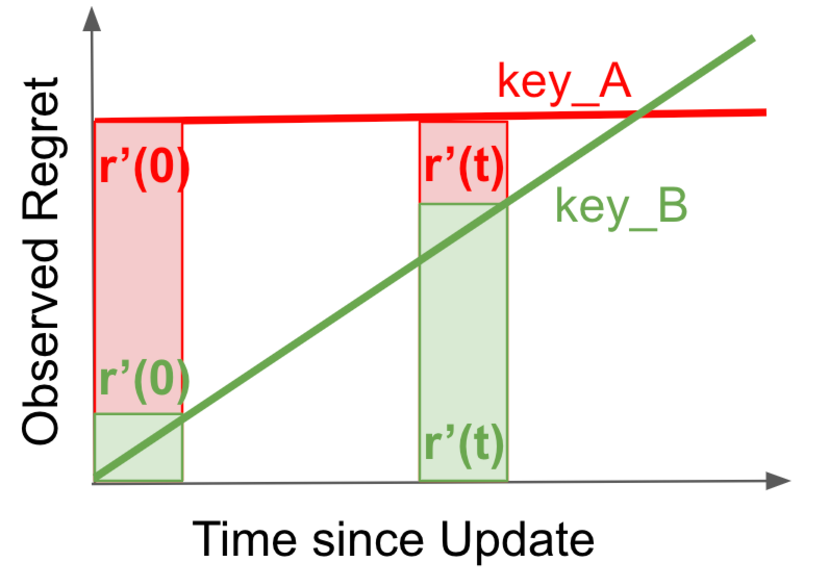
\includegraphics[width=8cm]{ralf/figures/r_tmp.pdf}
\setlength{\belowcaptionskip}{-10pt}
\setlength{\abovecaptionskip}{10pt}
\caption{}
\label{f:overview}
\end{figure}

\subsubsection{Policy Regret}

\begin{equation*}
u_{k,t} = \begin{cases}
t &\text{if $k \in U_t$}\\
u_{k,t-1} &\text{o.w.}
\end{cases}
\end{equation*}

Let $p_{t,k} = m(x_{t,k}, f(\mathcal{D}_k^{t-s}))$ and $y_{t,k}$ be the true labels. 

\begin{equation}
    C(\delta_{k,t}) = \sum_{s=0}^{\delta_{k, t}} \ell(f(\mathcal{D}_k^{t-s}), f(\mathcal{D}_k^{t-\delta_{k,t}}))
\end{equation}

Say we have queries $\{x_i\} \in Q_{t,k}$ for queries using key $k$ at timestep $t$, which correspond to an unknown set of true labels $\{y_i\} \in Q_{t,k}$.  At a later time, we receive prediction errors $\{e_i\} \in E_{t,k}$ corresponding to each query.  

For a feature $\tilde{v}_k^t$, we can estimate regret as a function of $\delta_{k,t}$:
\begin{align}
    e_k(s) &= \mathbb{E}_i\left[\ell\left(m(x_i, f(\mathcal{D}_k^{t-\delta_{tk}})), y_i\right)\right] \\
    &\approx \sum_{\{e_i\} \in E_{u_{t,k} + s,k}} e_i
\end{align}
We define the cumulative regret for a feature $\tilde{v}_k^t$
\begin{equation}
    r_k(\delta) = \sum_{s=0}^{\delta_{tk}} e_k(t-s) - e_k(t-{\delta_{tk}})
\end{equation}


\subsubsection{Online Regret Estimation}
We can maintain a sum of the regret observed since a feature value $\tilde{v}_k$ was last updated. We denote the function $r_k(\delta)$ which is the cumulative regret with update delay $\delta$ for key $k$. 
\begin{equation}
   r_k(\delta) = \mathcal{R}(\tilde{v}^{t_u}; \mathcal{D}^{t_u+\d elta})
\end{equation}
We define the \textit{policy regret} as the cumulative sum of the error 
\begin{equation}
    \mathcal{C}(\tilde{v}^{t_u}; \mathcal{D}^{t_u+\delta}) = \sum_{s=0}^\delta (r_k(s) - r_k(0))
\end{equation}

We can estimate the expected total regret at timestamp $t+a$ using a first order Taylor expansion: 
\begin{equation}
    r_k(\delta + t) \approx  r_k(
    \delta) +r_k'(\delta)\cdot(t+\delta)
\end{equation}
We can use this to estimate the future regret incurred from an update to make scheduling decisions. 

\subsubsection{Scheduling Policy}
We propose an online scheduling policy where we prioritize keys based off which keys have the highest expected regret, which we estimate with a first order approximation. 

At a high-level, we use the measured regret over past time intervals to estimate the relationship between staleness and regret for different keys. 


If we do not update at time $t$, the expected future error is: 
\begin{align}
   \sum_{t'=t}^T\mathcal{R}(\tilde{v}^{t_u}; \mathcal{D}^{t'}) &= r_k(T-t_u) - r_k(t-t_u) \\
   &= r'_k(t-t_u)(T-t)
\end{align}
If we do update at time $t$, our last update time is $t$, so the expect future error is: 
\begin{align}
\sum_{t'=t}^T\mathcal{R}(\tilde{v}^{t}; \mathcal{D}^{t'}) &= r_k(T-t) \\
&= r_k(0) + r_k'(0)(T-t)
\end{align}
We can set $r_k(0)=0$ and take the difference between the errors with and without updating to obtain: 
\begin{align}
&\sum_{t'=t}^T\mathcal{R}(\tilde{v}^{t_u}; \mathcal{D}^{t'}) - \mathcal{R}(\tilde{v}^{t}; \mathcal{D}^{t'}) \\
&= 
    \left(r_k'(t-t_u) - r_k'(0)\right)(T-t) - r(0)
\end{align}
\sarah{Note: we are assuming that the last feature update r(0) is the same r(0) for future feature updates}
Given a function $u_k(t)$ mapping to the last update time for a key $k$, we can assigned key priorities proportional to the total expected regret as: \textcolor{red}{TODO: add query distribution}
\begin{align}
    p_k(t) \approx r_k'(t-u_k(t)) - r_k'(0) 
\end{align}

If we set a window $w$ to be equal to the featurization runtime (the interval that scheduling decision are made) and only consider the next $w$ time interval, we can simplify the equation to simply equal the cumulative regret observed in the most recent $w$ window minus the cumulative regret observed in the window right after fitting the feature. 
\begin{align}
    p_k(t) \approx \sum_{t'=t}^{t- w} \mathcal{R}(\tilde{v}^{t_u}; \mathcal{D}^{t'}) - \sum_{t'=t_u}^{t_u+ w} \mathcal{R}(\tilde{v}^{t_u}; \mathcal{D}^{t'})
\end{align}

% We want to identify the key which will give us the greatest reduction in error between the current timestamp $t$ and $T$. \begin{equation}
%     r_k(T-t_u) -  r_k(t-t_u) \approx \frac{d}{dt}r_k(t-t_u)\cdot(T-t)
% \end{equation}
% We can approximate $\frac{d}{dt}r_k(t)$ with observations of the cumulative error and definining a window size $\delta$:
% \begin{equation}
%     \frac{d}{dt}r_k(t) \approx \frac{1}{\delta} (r_k(t) - r_k(t-\delta))
% \end{equation}
% If we assume discret timesteps, we can approximate  $\frac{d}{dt}r_k(t)$ as:
% \begin{equation}
%     \frac{d}{dt}r_k(t) &=& \mathcal{R}(\tilde{v}^{t_u}; \mathcal{D}^{t_u+t}) 
% \end{equation}




\subsubsection{No starvation} we can prevent starvation by upper bounding the regret $\mathcal{R}_{max}$, so $\frac{d}{dt}r_k(t) \le \mathcal{R}_{max} \forall k, t \in [0, T)$. 

\subsubsection{Optimality} \textcolor{red}{The scheduling policy is optimal within some bound of error}. Assuming a perfect estimate of the cumulative error, greedily choosing the update with the largest regret improvement is optimal. The first order approximation is correct within the bound (???).  

% \subsubsection{Formulation}
% We formalize the scheduling problem as given a constraint $C$ on the number of featurization updates which can be performed in some time interval $T$, select a subset of pending events $\{e_{k,i}\}$ process within that constraint to minimize feature store regret.  
% \begin{equation}
%     |\{e_{k,i}\}| \le C, \{e_{k,i}\} \in D_k^t
% \end{equation}
% We denote the set of keys corresponding to the chosen events at timestemp $t$ as $K_t$. We assume the featurization step will complete in $\delta$ timesteps, so the next version of the feature table values can be written as:  
% \[
%     \tilde{v}^{t+\delta} = 
% \begin{cases}
%     f(\mathcal{D}_k^t),& \text{if } k\in {K_t}\\
%     \tilde{v}^t,              & \text{otherwise}
% \end{cases}
% \]
% We can write the objective of the scheduler as choosing $\tilde{v}^{t+\delta}$ which minimizes the feature store regret at time ${t+\delta}$:
% \begin{equation}
%     \argmin_{\tilde{v}^{t+\delta}} \mathcal{L}(\tilde{v}^{t+\delta}; \mathcal{D}^{t+\delta})
% \end{equation}

% We note that we formulate the scheduling problem as a \testit{greedy} scheduling problem, as we assume we do not have visibility 


% \subsection{Formulation}
% We formulate the scheduling problem as solving an update matrix $U$. We define $U$ as:
% \[
%     U_{t,k,v} =  
% \begin{cases}
%     1,& \text{if } \tilde{v}_k^t = f(\mathcal{D}_k^v) \\
%     0,              & \text{otherwise}
% \end{cases}
% \]

% The optimal update matrix: 
% \[
%     U^*_{t,k,v} =  
% \begin{cases}
%     1,& \text{if } v = t \\
%     0,              & \text{otherwise}
% \end{cases}
% \]

% We can multiple the update matrix with a matrix $F$ containing feature versions at every timestep $v$: 
% \begin{equation}
% F_{k,v} = f(\mathcal{D}_k^v)  
% \end{equation}

% We can denote the feature store regret as: 
% \begin{equation}
%     \mathcal{R} = \mathcal{L}(UF, U^*F)
% \end{equation}
% Given a convex loss function $\mathcal{L}$, the feature store regret $\mathcal{R}$ is convex with respect to $U$. Therefore, using a greedy scheduling mechanism to determine $U$ online will minimize $\mathcal{R}$. 



% We formalize the scheduling problem as choosing key priorities $[p_1, p_2, ... p_n]$ for keys $[k_1, k_2, ...k_n]$. 

\subsection{Estimating Feature Store Regret}
Our policy relies on having a measure of aggregate feature store regret over time intervals. While we define \eqref{eq:feature-store-regret} to be computatable without access to prediction labels (which are often not available)

\subsubsection{Ground-Truth Labels}

\subsubsection{Predictions with Complete Features}

\subsubsection{Application-specific Heuristics}




The two factors affecting whether a key is important to update are: (1) the query importance (how frequently is the feature queried for downstream predictions?), and (2) prediction degradation (how likely is the feature to return similar prediction as the optimal version of the feature?). (1) is simple to infer from query patterns over the feature table, while (2) depends on multiple factors, such: 
\begin{enumerate}
    \item Staleness: Staler features are more likely to be lacking recent data. 
    \item Rate of change: Features which are changing faster than others are more likely to hurt predictions than feature values which are relatively constant. 
    \item Significance of new data: Some updates are less likely to affect a feature value than others. For example, a feature representing an average user purchase from thousands of purchases is much less likely to have large feature regret as compared to one computed from just a few data points.
\end{enumerate}


\jmh{Seems like you could narrate more here. An ideal feature store is always up-to-date with all data updates, and our goal is to approximate that effect despite some updates being skipped or delayed. In that setting, we want to characterize an application-specific notion of the error---regret---that we observe due to the feature store not reflecting the latest updates. To that end, we will characterize the error for each query in some workload relative to the ideal, and then an overall metric of the error for that workload as a whole.}


% The feature store queries $Q$ are sent by downstream models, where each $(d, k, t) \in Q$ contains query data $d$ \jmh{I thought $d$ was a data update! Maybe pick distinguished variables for updates and queries.}, feature key $k$, and timestamp $t \in (0, T]$ at which the query is sent. Model predictions are generated from the query data and current feature value with $m(d, v_\phi^{(t)}(k))$. 

% We use the downstream model's \textit{loss function} $\ell$ to quantify the distance between model predictions for different policy parameters $\phi$. For a query $(d, k, t) \in Q$, we can measure the difference \sarah{idk whether to call this difference or distance} between prediction outputs for two different featurization policy parameters $\phi, \phi'$ as:
% \begin{equation}
%     \mathcal{D}(d, k, t, \phi, \phi') = \ell(m(d,  v_{\phi}^{(t)}(k)), m(d,  v_{\phi'}^{(t)}(k)))
% \end{equation}

% We define \textit{feature store loss} for policy $\phi$ as the average distance \jmh{Seems like you could/should generalize to different metrics beyond average ($L_2$ norm)} $\mathcal{D}$
% %\kevin{distance by what metric?} 
% the optimal policy parameters $\phi^*$ and $\phi$ over a set of queries $Q$. We can write the feature store loss \kevin{how about "feature schedule regret" the name for this? i think regret, like in RL conveys that this is the difference between our policy and the oracle policy} for policy parameters $\phi$ and queries $Q$ as:
% \begin{equation}
% \mathcal{L}_{F}(\phi, Q) = \frac{1}{|Q|}\sum_{(d, k, t) \in Q} \mathcal{D}(d, k, t, \phi^*, \phi)
%     %\mathcal{L}_{FS}(\phi, Q) = \frac{1}{|Q|}\sum_{(d_q, k_q, t_q) \in Q} \mathcal{L_P}(\hat{m}(d_q,  v_{\phi_{opt}}^{(t_q)}(k_q), \hat{m}(d_q,  v_\phi^{(t_q)}(k_q)))
% \end{equation}
% %\sarah{joey: maybe only do one parameters?}
% The optimal parameter policy $\phi^*$ represents the parameters for computing features optimizing only for downstream accuracy and without consideration for cost or feasibility.
% \natacha{Two things:
% 1) this is Eurosys, go easy on the reader. What you're saying is not super complicated, but some intuition would help "soften" the maths 2) it's a bit comfusing to have phi be both the optimal parameter policy when phi* is always going to be compute on everything, and for slide size 1. The way you phrase it, it sounds like it might not be optimal to compute on every input. You also define phi* twice here}



%Features also allow for models to leverage real-time information in making predictions\sarah{cite:uber}. Data and features used for training are usually generated from historical data, so features maintained over time provide the model with time-dependent information when making a prediction. For example, a recommendation model may use features representing a user’s recent behavior on an e-commerce site, e.g. the user’s last 5 clicks, to make predictions accounting for real-time context.
%\natacha{I would keep this section and remove the ones that you have above (except for the online training description). I would "merge" the formula that you have above into this paragraph, but the rest of the text is pretty redundant with what you have here}

%\subsubsection{Online/Offline Store}
%Features are often pre-computed and cached in a data store to save on feature computation time and to avoid redundant featurizations. For online prediction serving, features are often too expensive to compute on-request and the same features may be used across different predictions. For example, a recommendation model may be run many times for a single user, and use the same user preference feature for each prediction. 
%Features are often pre-computed and cached in a data store, typically referred to as the \textit{offline store} for features used during training and the \textit{online store} for features using during inference. Caching features eliminates redundant computations across model predictions using the same features, and reduces the amount of computation that needs to be done on-the-fly, such as when a prediction request is made to a model. 




%Feature stores typically contain two separate data stores for features used during model training versus model serving, the \textit{offline store} and \textit{online store}, due to varying system requirements. Tight latency constraints for online prediction serving (<100ms) require inference-time features to be stored in a low latency data stores (e.g. Redis, Postgres), while train-time features are preferably stored in a higher-latency, more durable data store (e.g. S3, BigQuery). 
% \simon{actually not quite, online is real-time and serving current set of feature, it doesn't need to be in-memory but it should be low latency. for example Postgres can totally be used online; on the other hand, offline is there to store historical data for training plus data doesn't need to be in online store}




% \subsubsection{Feature Maintenance Policy Parameters}
% \label{s:policy-parameters}
% In general, there are many ways to implement data dependent delays $\delta(\mathcal{D}^t_k)$ and sampling $s(\mathcal{D}^t_k)$.  
% To simplify further notation we will define \emph{feature maintenance policy} parameters $\phi_k$ as a vector of parameters associated with each key that determine the specific details of the delay or sampling policy associated with key $k$.  
% For example, these parameters might include the slide size as well as the window size for a sliding window feature function.
% In addition, $\phi_k$ may define key sampling parameters like the rate or bias towards recency.
% %\natacha{define each term}
% %\natacha{This is the first time you've talked about load shedding}
% More concretely, if we choose slide size $12$ and sub-sampling rate $0.5$ for key $k=1$, we have $\phi_1=[12, 0.5]$. \jmh{Consider a concrete plausible running example for all your ``more concretely'' things, or the places where I asked for examples. Ideally also your system's API syntax for specifying the $\phi$ parameters realistically.}





. 




\jmh{I worry as a reader that your notion of parameters per key may not capture some more elaborate schemes that I haven't thought of yet. Like maybe you know correlations across keys and you featurize across them in some interdependent way. Is it necessary for your work to have $\phi$ defined crisply? Are there kinds of policies you will need to rule out?

\subsection{The Feature Maintenance Problem}
% \joey{Consider making this a section instead of a sub section.}
% \subsection{Feature Maintenance Cost}
While our goal is to minimize the feature store loss by employing a combination of the mechanisms described in Section \ref{sec:mechanisms}, we are constrained by the available resources and the associated cost of feature updates. We define the problem of feature store maintenance as choosing \textit{feature maintenance policy parameters} to minimize loss under resource constraints.  We estimate these parameters by observing resource costs and feature store loss with historical data for $\mathcal{D}^t$ and the observed historical query distribution $Q$.




\subsubsection{Optimizing the Feature Maintenance Policy} 
We can select the optimal feature maintenance policy $\phi$ by minimizing the feature store loss under cost constraints for maintaining feature values. 
We can define $c(k, \phi_k, \mathcal{D}^t_k)$ as the cost of \emph{approximately} maintaining the feature table entry $\tilde{v}^t_k$ as a function of the data $\mathcal{D}^t_k$ associated with that key $k$ as well as our choice of policy parameters $\phi_k$.  Given the above notation for the feature store loss and the feature cost we can formally define the feature store maintenance problem as a constrained optimization problem of the following form:
\begin{align}
& \arg\min_{\phi}  \sum_{t=1}^T 
    % \sum_{k=1}^K
    % \mathbb{E}_{k\sim Q}\left[\ell\left(
    % m\left(x, f\left(\mathcal{D}^t_k \right)\right),
    % m\left(x, \tilde{v}^t_k \right)
    % \right)\right]
   \mathcal{L}\left(\tilde{v}^t; \mathcal{D}^t\right)
\\
& \text{s.t.} \quad  \forall t: \,\, \sum_{k=1}^K c\left(k, \phi_k, \mathcal{D}^t_k\right) < C
\end{align}
where $K$ is the number of keys, $T$ is the duration of time for which we have data, and $C$ is the cost constraint (e.g., the number of feature updates that can be performed).
The constraint term ensures that for ever time interval the amount of resources required is within the resource budget. 
We use a numerical optimizer \jmh{what, specifically? or fw ref to further discussion below?} to determine the best policy parameters for each key, which can be used to configure feature maintenance policies to improve downstream accuracy.  \jmh{the second half of this sentence didn't really make sense to me... is it just ``so we can follow that policy?''?}

\jmh{Seems like there's a big independence assumption here across keys! Do you want to acknowledge that here and add a discussion (either here or below with a fw ref?}

\subsubsection{Estimating Cost and Loss}


%We denote the ideal, high-cost feature parameters as $\phi^*$, which we assume will maximize downstream accuracy. For example, for slide size and sampling parameters, $\phi^*_k = [1, 1]$ as those parame ters result in the least stale and most accuracy \natacha{Phrasing is odd. Why would $\phi_k$ have a parametrisable slide size or sampling parameter? isn't it always 1, 1?}. 

%Unfortunately, the feature maintenance problem depends on the distribution of data arrivals $\mathcal{D}^t$ as well as the query distribution $Q$.
%We adopt an empirical approach and use historical data for $\mathcal{D}^t$ and the observed historical query distribution $Q$.



\joey{We need to say more about how we actually solve this problem.  I noticed in the text that we allude to an LP but the loss is probably quadratic or at least not linear so that is concerning...}


We estimate the feature store loss $\mathcal{L}$ and cost $c$ by running simulations with various parameter values using historical data $\mathcal{D}^t$ and queries $Q$. The precise value of $c$ can be measured in terms of compute resources or approximated as the number of feature updates performed, in cases where the feature function is the primary bottleneck. We consider the true feature values $f(\mathcal{D}_k^t)$ (for measuring feature store loss in \ref{eq:feature-store-loss}) to be the features computed in the absence of computational constraints, such as slide size or sampling rate 1 (which we assume will maximize accuracy). 

\important{Can we say a bit more about how $c$ might be measured in practice here?}

% In order to constrain the search space for $\phi$, we make two simplifying assumptions %\jmh{Aha -- I smelled these assumptions above before you stated them. I recommend you start with the most general characterization up above, and then constraint/reformalize it here, with a nod to a future work section that will examine relaxing these. Then you get full credit for setting up the problem even if somebody else writes the follow-on.}:
% \begin{enumerate}
%     \item \textit{Cross-Key Independence.} We assume key-level policies $\phi_k$ can be determined independently by computing $c$ and $\mathcal{L}$ separately for each key.  
% % \begin{eqnarray}
% % C_{F}(\phi, E) &=& \sum_{k\in K}  C_{F}(\phi_k, E) \\
% % \mathcal{L}_{F}(\phi, Q) &=& \sum_{k\in K} \mathcal{L}_F(\phi_k, \{(d, k', t)\in Q| k' = k\})
% % \end{eqnarray}
% \item \textit{Discrete Parameter Options.} We require each individual parameters $\phi_{ki}$ to be limited to $\phi_{ki} \in \tau_i$ where $\tau_i$ is a set of possible options for parameter $i$. Therefore, the number of possible policy options for each key is equal to $\prod_{i=0}^n |\tau_i|$ for $n$ parameters.
% \end{enumerate}

% offline evaluation over a set of events $E$ and queries $Q$ within a previous time interval. We sample events $E$ and queries $Q$ from a prior time interval to evaluate the featurization loss $\mathcal{L}_F$ for different policies by calculating the cost and downstream accuracy for each $\phi$ and $\phi^*$. 






